\section{Versuchsaufbau und Durchführung}
\label{sec:Aufbau}

Die eintreffenden Myonen werden mit einem Szintillatortank registriert. Diese erzeugen einen Lichtblitz, wenn sie eintreffen. Daraufhin wird dieser durch Photomultiplier kurz PMT in einen messbaren Strom umgewandelt, ähnlich wie der Photoeffekt und zusätzlich verstärkt. Der Spannungspuls wird anschließend als Eingangssignal für eine Messschaltung verwendet, die zur weiteren Verarbeitung dient.

\subsection{Aufbau}
Um eine visuelle Vorstellung zu erlangen, wird der Versuchsaufbau grob mithilfe von Fotos, die selbst aufgenommen wurden in Abbildung \ref{fig:1} und \ref{fig:2} dargestellt.\newline 

\begin{figure}[H]
\centering
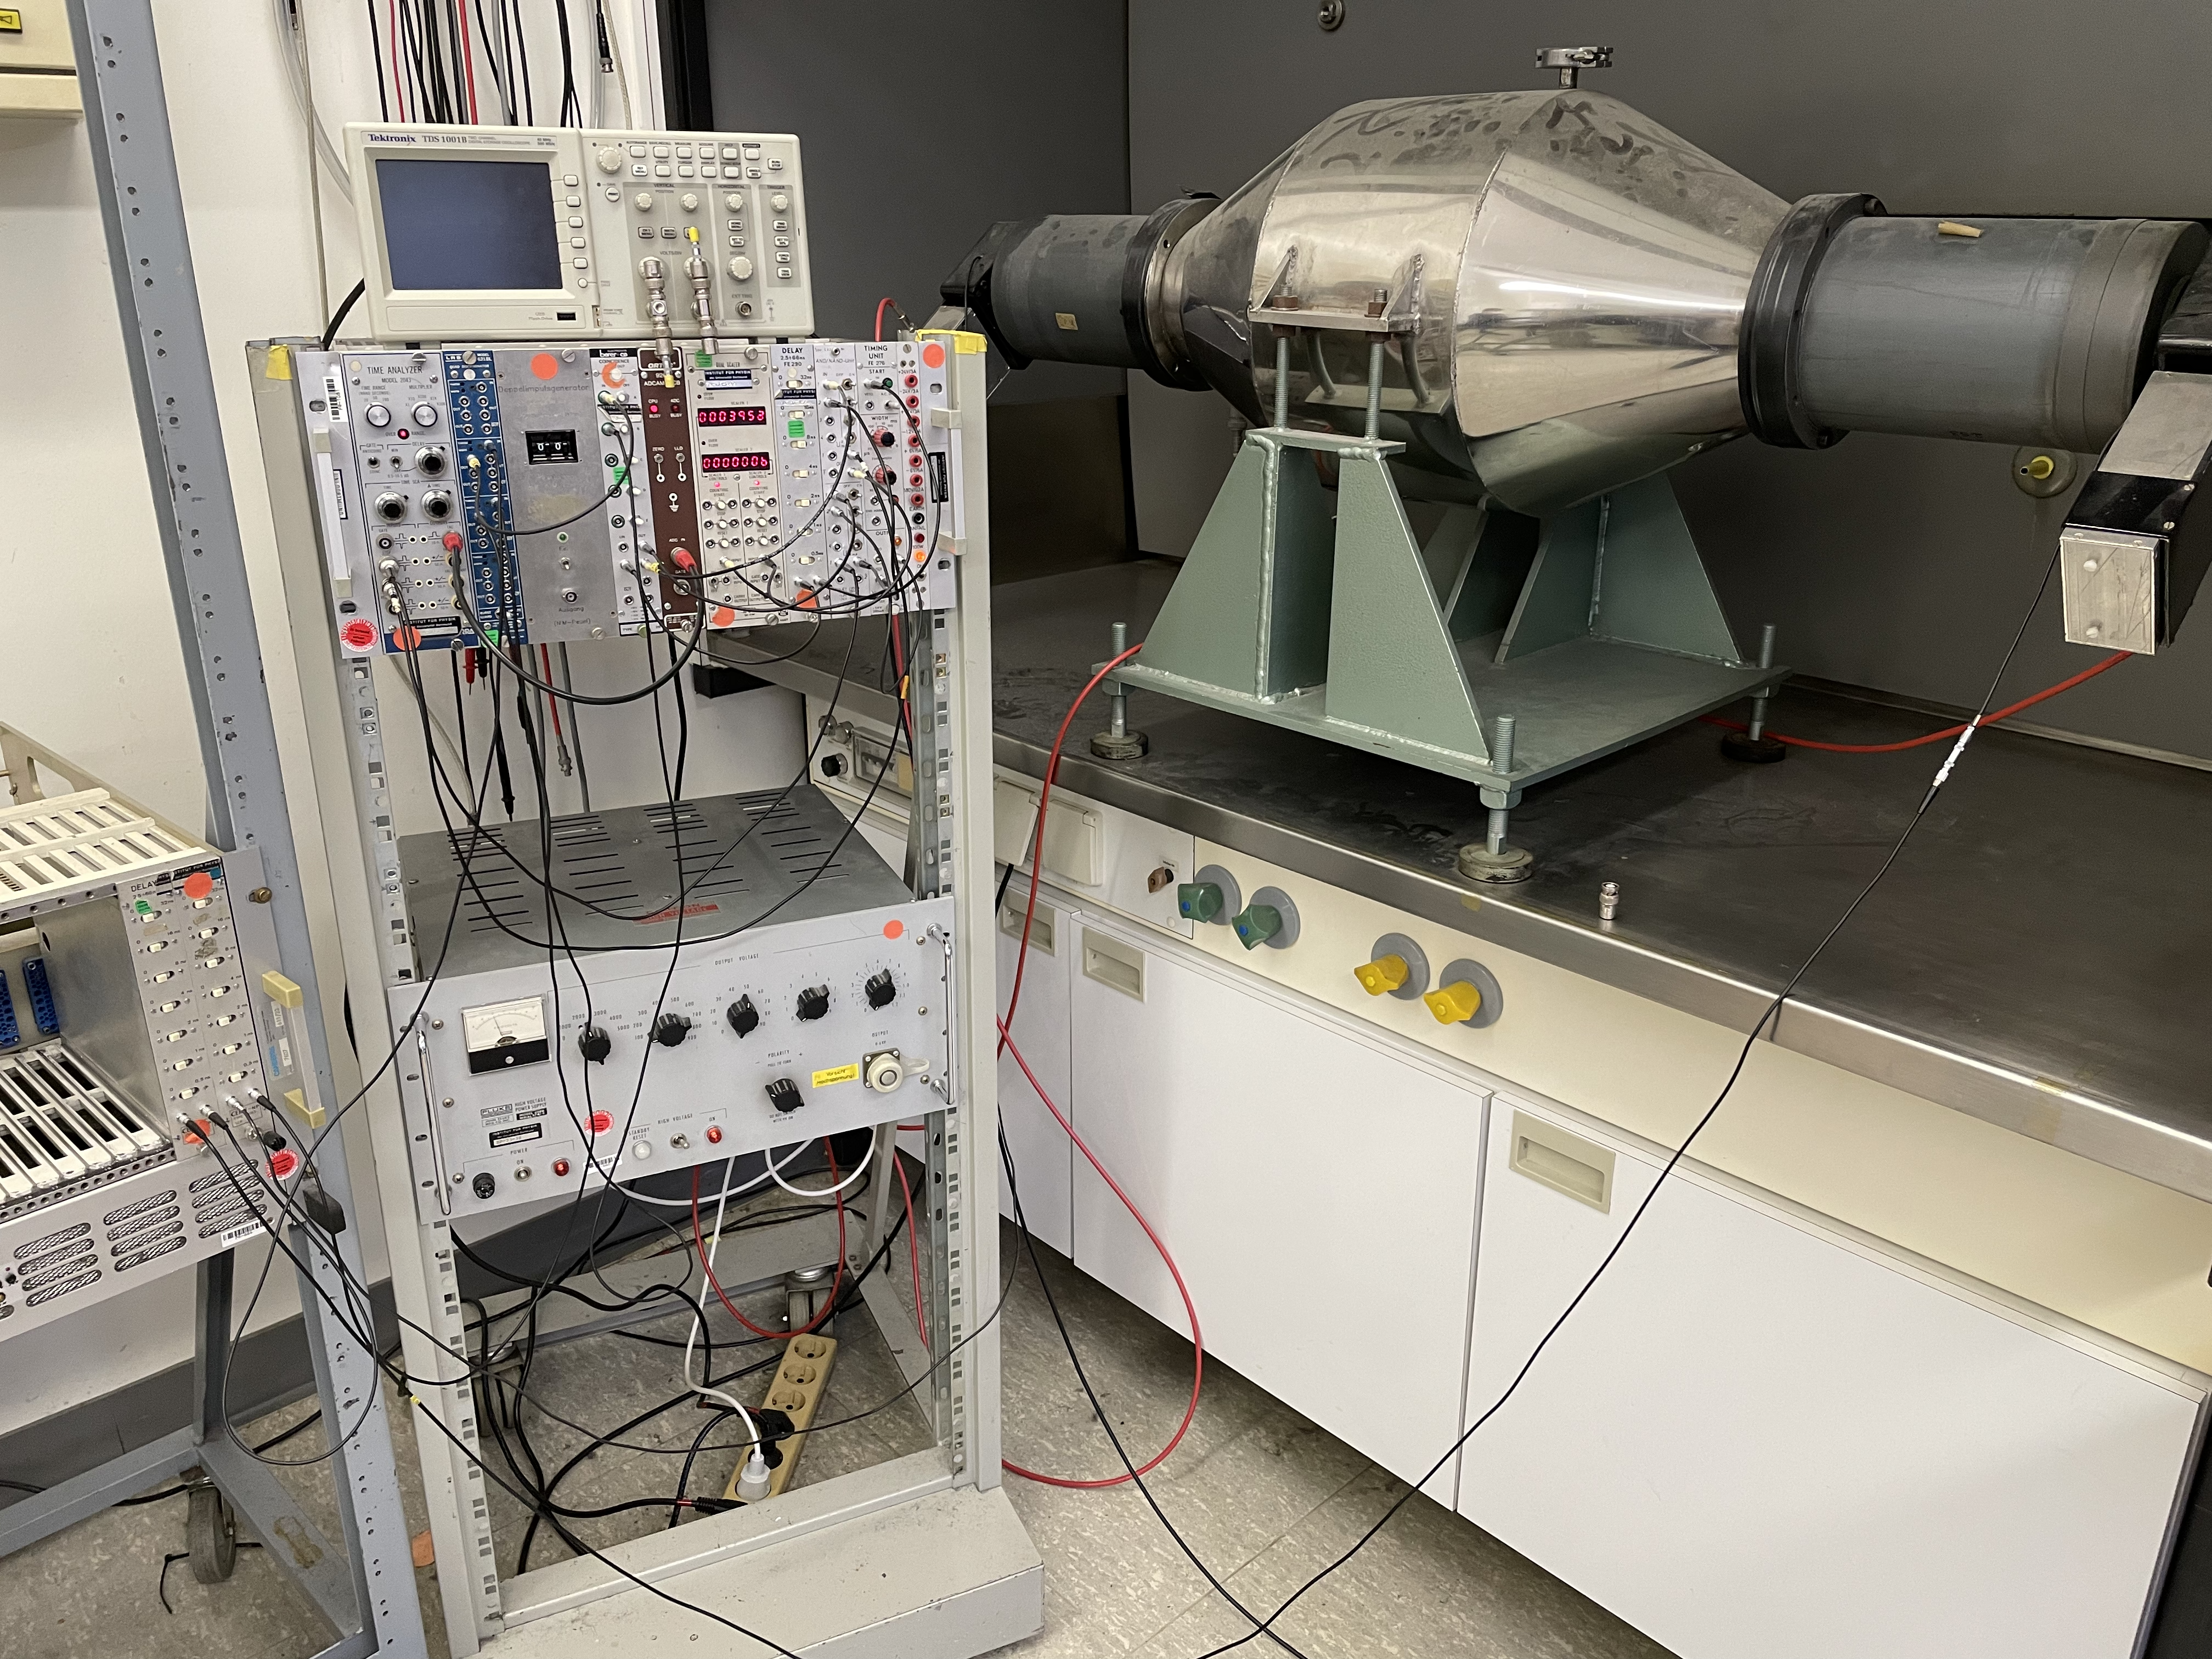
\includegraphics[scale=0.1]{1.jpg}
\caption{Erstes Foto zum Versuchsaufbau. Rechts: Szintillator mit Photomultiplier.}
\label{fig:1}
\end{figure}

\begin{figure}[H]
\centering
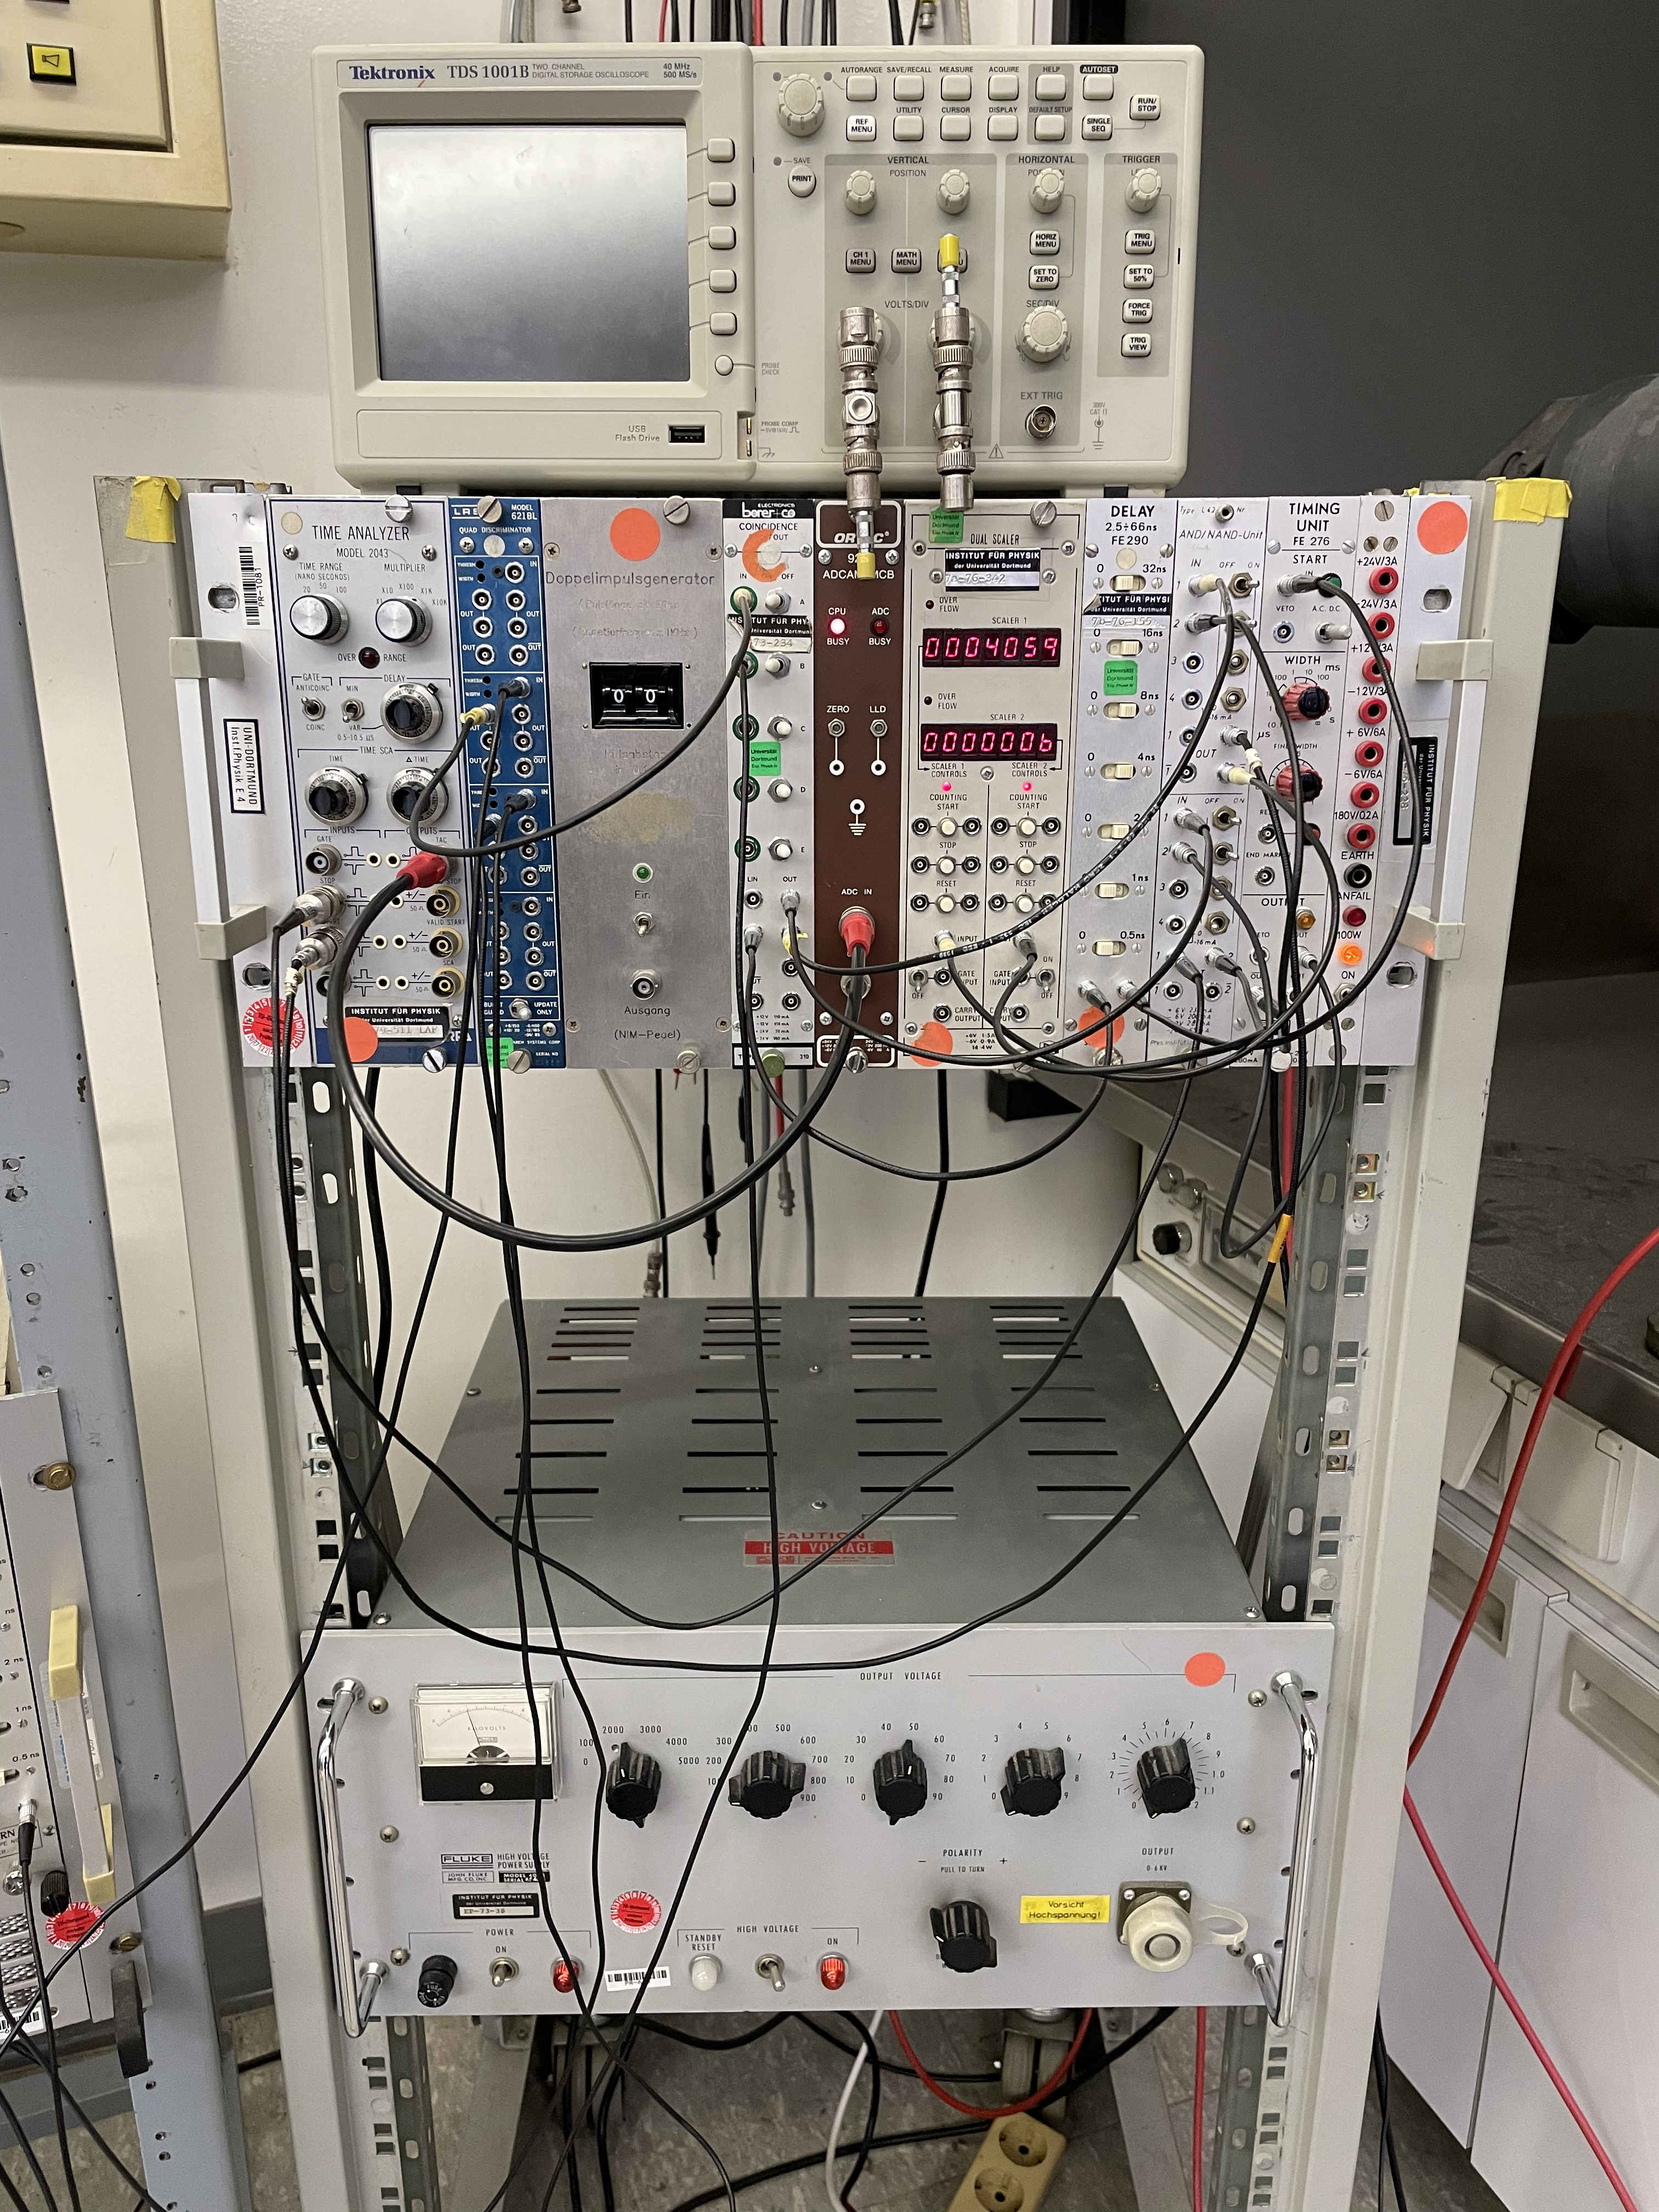
\includegraphics[scale=0.1]{2.jpg}
\caption{Zweites Foto zum Versuchsaufbau. Das Oszilloskop und darunter die einzelnen Bauteile.}
\label{fig:2}
\end{figure}

\noindent Der Versuchsaufbau besteht aus einem Szintillator mit einem Tank, der ungefähr ein Volumen von 50 l erfasst. An den beiden Enden des Tanks ist je ein Photomultiplier kurz PMT befestigt. Die Ausgänge der einzelnen PMT werden über eine Verzögerungsleitung auf den Eingang eines Diskriminators mit variabler Schwelle gesteckt. Dieser filtert die ankommenden Signale so, dass das unterschwellige Rauschen verschwindet. Das Ausgangssignal wird dann so moduliert, dass unter Berücksichtigung der Lichtlaufzeit im Szintillator alle Myonen unabhängig von wo sie eintreten, verknüpft werden können. Zusätzlich einstellbar ist die Pulsdauer am Ausgang der Diskriminatoren. \newline 
\newpage 
\noindent Die beiden Signale werden in eine Koinzidenschaltung weitergeleitet. Diese erzeugt nur ein Ausgangssignal, wenn die Pulse zeitgleich an ihrem Eingang eintreffen. Als nächstes folgt das elektronische Äquivalent einer Stoppuhr. \newline
\noindent Das Ausgangssignal der Koinzidenz wird weitergeleitet zu zwei AND-Gattern sowie über eine zusätzliche Verzögerungsleitung mit $\symup{\increment t= 30} \mathrm{ns}$ zu einem sogenannten Monoflop. Dieser Monoflop wird auch Univibrator oder monostabile Kippstufe genannt. Dieser dient dazu die Suchzeit $\symup{T_s}$ vorzugeben. Die AND-Gatter sind mit dem Time-Amplitude-Converter kurz TAC verbunden, welches zum einen die Zeitmessung startet, während das andere diese stoppt. Die zusätzliche Verbindung zu den einzelnen Impulszählern dient dazu die Start- und Stoppimpulse zu zählen. \newline
\noindent Mithilfe einer geeigneten Kombination der Bauteile kann die Zeitmessung gestartet werden, wenn das Myon das aktive Volumen des Szintillisators betritt. Sobald das Myon zerfällt, wird die Messung gestoppt.\newline
Das Signal, welches aus dem TAC herauskommt, gelangt in den Vielkanalanalysator. Dieser wird auch Multi-Channel-Analyser (MCA) genannt. Mithilfe eines PCs und einer installierten Messsoftware werden die Signale ausgelesen. Für die Kalibration des MCA wird ein Doppelimpulsgenerator verwendet. Dieser generiert Doppelimpulse mit einem variablen Zeitabstand bei einer Frequenz von 1 $\mathrm{kHz}$. \newline
\noindent In der nachfolgenden Abbildung \ref{fig:Schaltbild} ist das Schaltbild des Versuches dargestellt.

\begin{figure}[H]
\centering
\includegraphics[scale=0.7]{Schaltbild.pdf}
\caption{Schaltbild der Messapparatur. [5]}
\label{fig:Schaltbild}
\end{figure}
\newpage
\subsection{Der Szintillator}
\label{sec:Szintillator}
Der Szintillator besitzt einen Tank mit einem organisch, gelösten Szintillat. Sobald ein Myon auf dieses Material trifft, regt es einige Moleküle in diesem Szintillator an, die letzendlich dazu führen, dass bei der Rückkehr in den Grundzustand Photonen emittiert werden. Diese liegen im sichtbaren bis hin zum nahen Ultravioletten Bereich des Spektrums. \newline
\noindent Zusätzlich erzeugt der Zerfall des Myons einen Lichtblitz im Szintillatortank. Der zeitliche Abstand zwischen Eintritt und Zerfall entspricht der individuellen Lebensdauer eines Myons. Somit ist der Szintillationsdetektor zur Bestimmung der Lebensdauer  von Myonen bestens geeignet.

\subsection{Der Photomultiplier (PMT)}
\label{sec:PMT}
Um die geringen Energien der Lichtimpulse analysieren zu können, müssen diese verstärkt werden. Dazu dienen die Photomultiplier. Die Photonen treffen auf eine Kathode. Aus dieser lösen sich einzelne Elektronen aus (Photoeffekt). Beim Anlegen einer Hochspannung werden diese innerhalb des PMT zu hintereinander geschalteten Elektroden hin beschleunigt. Aus diesen werden weitere Elektronen ausgeschlagen, die eine messbare Menge an Elektronen erzeugen. 

\subsection{Fehlerquellen und die Untergrundrate}
\label{sec:Untergrundrate}
Die Photomultiplier neigen dazu spontan Elektronen zu emittieren aufgrund der endlichen Temperatur. Obwohl kein Myon eingetreten ist, werden trotzdem Spannungspulse beobachtet. \newline 
\noindent Damit dieses Phänomen nicht stattfindet, werden hinter den PET sogenannte  Diskriminatorstufen installiert, die die Spannungspulse erst ab einer bestimmten Impulshöhe weitergeben und direkt an ihrem Ausgang dementsprechend weiterleiten. Es können jedoch weiterhin zufällige Signale mit einer Amplitude auftreten, die einem Myon-Einfall entsprechen. Deshalb werden zwei PMTs verwendet. Die Elektronenemission ist unkorreliert und somit ist es unwahrscheinlich, dass beide PMTs zeitgleich einen Impuls liefern. Die durch Myonen entstehenden Impulse werden gleichzeitig an beiden PMTs beobachtet (Verzögerung in $\mathrm{ns}$-Bereich). \newline
\noindent Das Eintreffen von zwei Myonen innerhalb der Suchzeit kann eine Fehlmessung erzeugen. Dadurch werden insgesamt mehr Counts registriert als tatsächlich eintreffende Myonen. Dieser Vorgang wird als Untergrundrate U bezeichnet. Diese wird in der Auswertung genauer erklärt und statistisch berücksichtigt (siehe Kapitel \ref{subsec:2}).

\subsection{Optimale Justierung}
\label{sec:Justage}
Eine sorgfältige Justage ist wie bei anderen Versuchen Voraussetzung für optimale Messergebnisse. Dabei muss einiges berücksichtigt werden.\newline
\noindent Die Photomultiplier können verschiedene Ansprechzeiten haben auch wenn sie die gleiche Bauart besitzen. Um diese Unterschiede auszugleichen wird der schnellere PMT mit einer Verzögerungsleitung angepasst und anschließend noch mit dem Diskriminator ausgeglichen. \newline
\noindent Bei der Koinzidenzapparatur wird am Univibrator die maximale Suchzeit eingestellt. \newline
\noindent Anschließend wird eine Kalibrierungsmessung mit dem Doppelimpulsgenerator an dem Vielkanalanalysator durchgeführt. Hierbei ist zu beachten, dass die Einstellungen so gewählt sind, dass möglichst viele der Kanäle des Vielkanalanalysators genutzt werden. Sprich beim Durchlaufen aller $\symup{t<T_s}$ sollte das letzte t, welches die Bedingung noch gerade so erfüllt, möglichst in einen der letzten Kanäle eingelesen werden.

\subsection{Durchführung}
\label{Durchführung}
Die Schaltung wird nach der Abbildung \ref{fig:Schaltbild} aufgebaut und ihre Funktion schrittweise vom Ausgang des Szintillationsdetektors bis zum Ausgang des TAC mithilfe eines Oszilloskopen überprüft. \newline
\noindent Die Photomultiplier werden mit Hochspannung versorgt. An den jeweiligen Ausgängen sollten Spannungsimpulse mit unterschiedlicher Höhe am Oszillographen zu sehen sein. Als nächstes werden die Schwellspannungen der Deskriminatoren so eingestellt, dass an beiden Ausgängen ungefähr 20 Impulse pro Sekunde gemessen werden. Die Impulsdauer wird auf 10 $\mathrm{ns}$ eingestellt. Dafür wird der Impulszähler angeschlossen. Für die Justage der Koinzidenapparatur werden systematisch je eine Verzögerungsleitung variiert. Dabei wird auf die Impulsrate am Ausgang der Koinzidenz geachtet. Der Messbereich sollte so gewählt sein, dass sich die Halbwertsbreite der Verteilung bestimmen lässt. Anschließend wird eine Verzögerung ausgewählt, die für die Dauer des Versuches eingestellt bleibt.\newline
\noindent Nun wird der restliche Teil der Schaltung verkabelt. Am Monoflop wird die Suchzeit $\symup{T_S}$ eingestellt und der Messbereich des TACs wird dementsprechend angepasst. Für die Kalibration des MCA wird der Doppelimpulsgenerator angeschlossen. Damit wird gemessen, welcher zeitliche Abstand der Doppelimpulse welchem Kanal des MCA entspricht. Die Kallibration wird mit mindestens zehn Messwerten im Bereich von 0,3 bis 9,9 $\symup{\mu s}$ durchgeführt. 
Zu guter Letzt werden die beiden PMTs angeschlossen und die Messung der Lebensdauer wird gestartet.